\chapter{Particle Reconstruction}
\label{sec:reco}

\section{The Tasks}

Our first problem, particle reconstruction, is a crucial part of any high-energy physics analysis. Here, we investigate an end-to-end ML model based on computer vision techniques, where we treat the calorimeter shower as a 3D image. Using a combined architecture, we simultaneously perform particle identification and energy measurement.

When dealing with particle reconstruction, one is interested in identifying a particle's type (electron, photon, etc.) and its momentum. An end-to-end application aiming to provide a full reconstruction of a given particle should thus be able to simultaneously solve a multi-class classification problem and a regression problem. In our study, we filter the REC dataset to make the classification task non-trivial, as described in Section~\ref{sec:data}. Since differentiating charged and uncharged particles is trivial, we judged the classification of our model on its ability to distinguish electrons from charged pions, and photons from neutral pions.

Our reconstruction networks were thus given the following three tasks:
\begin{itemize}
\item {\bf Identify electrons over a background of charged pions}: Charged pions are the most abundant particles produced in LHC collisions. They are typically located in jets, which are collimated sprays resulting from the showering and hadronization processes of quarks and gluons. On the other hand, electrons are rarely produced, and their presence is typically an indication of an interesting event occurring in the collision. A good electron identification algorithm should aim at misidentifying at most 1 in 10,000 pions as an electron. In order to increase the difficulty of our ML problem and to approach the kind of task that one faces at the LHC, we apply the HCAL/ECAL energy ratio cut as described in Section~\ref{sec:data}.
\item {\bf Identify photons over a background of neutral pions}: At particle colliders, the main background to photon identification comes from neutral pions decaying to photon pairs. In general, a generic $\gamma/\pi^0$ classification task is relatively easy, since the presence of two nearby clusters is a clear signature of $\pi^0$. Thus, we focus on events with high $\pi^0$ momentum, using the opening angle selection described in Section~\ref{sec:data}.
\item {\bf Energy measurement}: Once the particle is identified, it is very important to accurately determine its energy (and by extension, its momentum), since this allows physicists to calculate all the relevant high-level features, such as the mass of new particles that generated the detected particles when decaying. In this study, we address this problem on the same dataset used for the classification tasks, restricting the focus to range of energies from 2 to 500 GeV, and at various incident angles ($\eta$). Regression results using various neural network architectures were compared with results from linear regression, comparing both resolution and bias. The models we consider are designed to return the full particle momentum (energy, $\eta$, and $\phi$) of the incoming particle momentum. At this stage, this functionality is not fully exploited and only the energy determination is considered. An extension of our work to include the determination of $\eta$ and $\phi$ could be the matter of future studies.
\end{itemize}

\section{Baselines}

\subsection*{Classification Baseline}\label{app:BDT}

Boosted decision trees were chosen as the baseline of comparison for our classification task, due to their popularity in HEP experiments. Decision trees are effective in producing optimal cut-based decisions based on input features. A BDT is able to increase classification accuracy and stability by aggregating the results from multiple trees. Since a BDT optimizes cut selections, but still depends on the use of traditional pre-calculated features, we are able to use the BDT as a stand-in for standard HEP algorithms using feature-based cuts.

In a previous study~\cite{NIPS}, we compared the performance of a neural model taking energy cell info as input, a feature-based neural model, and a feature-based BDT. In that context, we demonstrated that feature-based BDTs and neural networks performed equally well. Thus, we do not compare feature-based neural networks in this paper, and instead only use feature-based BDTs to represent current state-of-the-art classification algorithms.

The features we use in our baseline BDT classification model~\cite{NIPS} are ones commonly used to characterize particle showers. One additional feature we added is R9, which measures the largest fraction of energy contained within a 3x3 window in a z-axis projection of the shower. This quantity provides a measure of the "concentration" of a shower within a small region. For values near 1, the shower is highly collimated within a single region, as in electromagnetic showers. Smaller values are typical of more spread out showers, as for hadronic and multi-prong showers. A comparison of R9 values between photons and neutral pions can be seen in Figure~\ref{fig:R9}, with examples of events with different R9 values being shown in Figure~\ref{fig:R9_examples}. After training, the discriminating power of various features can be seen in Figure~\ref{fig:BDT_ranking}.

\begin{figure}[htbp]
\centering
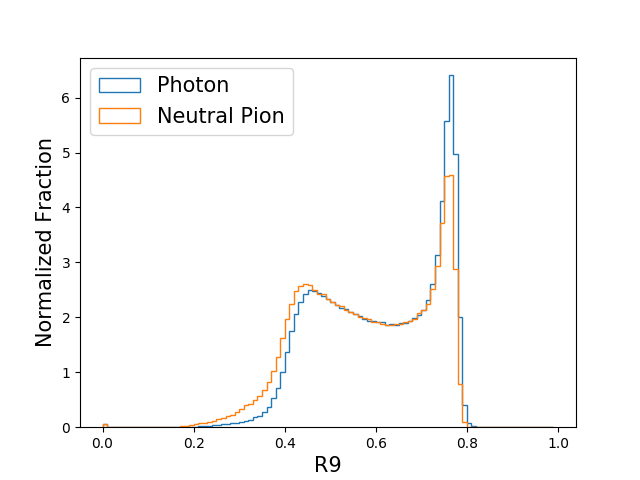
\includegraphics[width=0.6\textwidth]{Images/Calo/R9_ratios.png}
\caption{Comparison of R9 distributions between photon and neutral pion events. Photons tend to have more centralized energy depositions.
\label{fig:R9}}
\end{figure}

\begin{figure}[htbp]
\centering
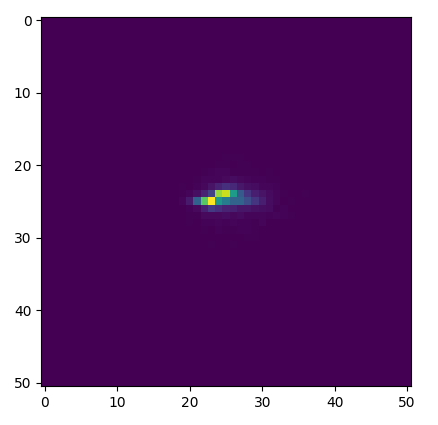
\includegraphics[width=0.4\textwidth]{Images/Calo/R9_0p42.png}
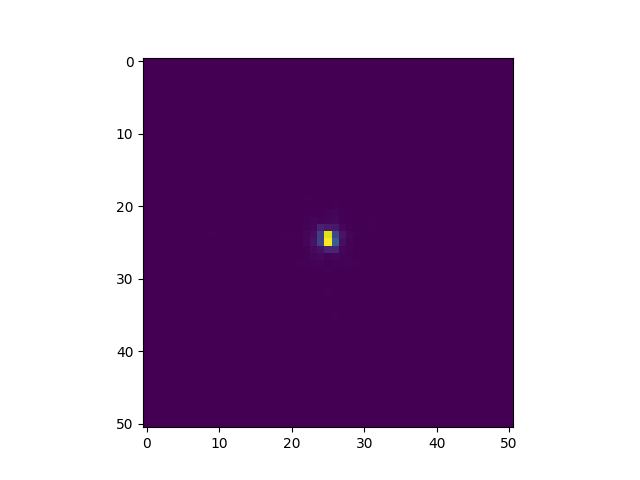
\includegraphics[width=0.4\textwidth]{Images/Calo/R9_0p75.png}
\caption{(Left) (x,y) projection of an event with R9=0.42. (Right) (x,y) projection of an event with R9=0.75.}
\label{fig:R9_examples}
\end{figure}

\begin{figure}[htbp]
\centering
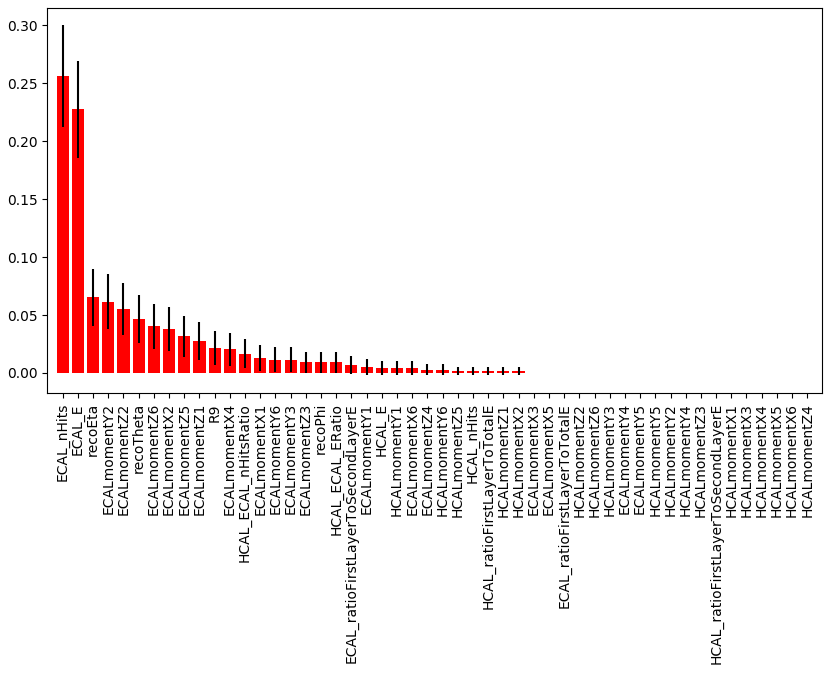
\includegraphics[width=0.7\textwidth]{Images/Calo/BDT_ranking_fixed.png}
\caption{Feature importances for inputs used in BDT training. Values shown are gini importances~\cite{Breiman}.\label{fig:BDT_ranking}}
\end{figure}

\subsection*{Energy Measurement Baseline}\label{app:regression_baseline}

We use linear regression as one of our energy measurement baselines, using ECAL and HCAL total energy as inputs, and where $a$, $b$, and $c$ are trained parameters:

\begin{equation}
E = a \cdot E_{ECAL} + b \cdot E_{HCAL} + c
\label{eq:linreg}
\end{equation}

Linear regression results for each of the particle types are shown in Figure~\ref{fig:reg_linreg}. Each point in the plot represents the mean bias or resolution within an energy bin. In all resolution plots shown in this thesis, the points have been fitted with the following expected resolution function equation:

\begin{equation}
\frac{\sigma(\Delta E)}{E_{\text{true}}} = \frac{a}{\sqrt{E_{\text{true}}}} \oplus b \oplus \frac{c}{E_{\text{true}}}
\label{eq:res}
\end{equation}

\begin{figure}[htbp]
\centering
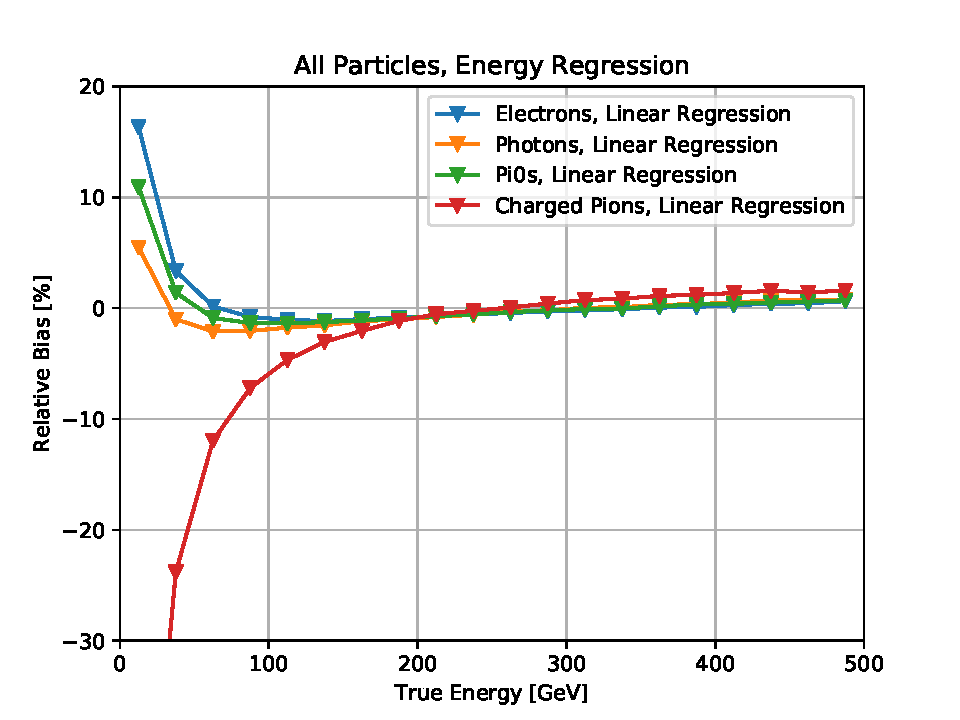
\includegraphics[width=0.45\textwidth]{Images/Calo/bias_vs_E_allparts_linreg.pdf}
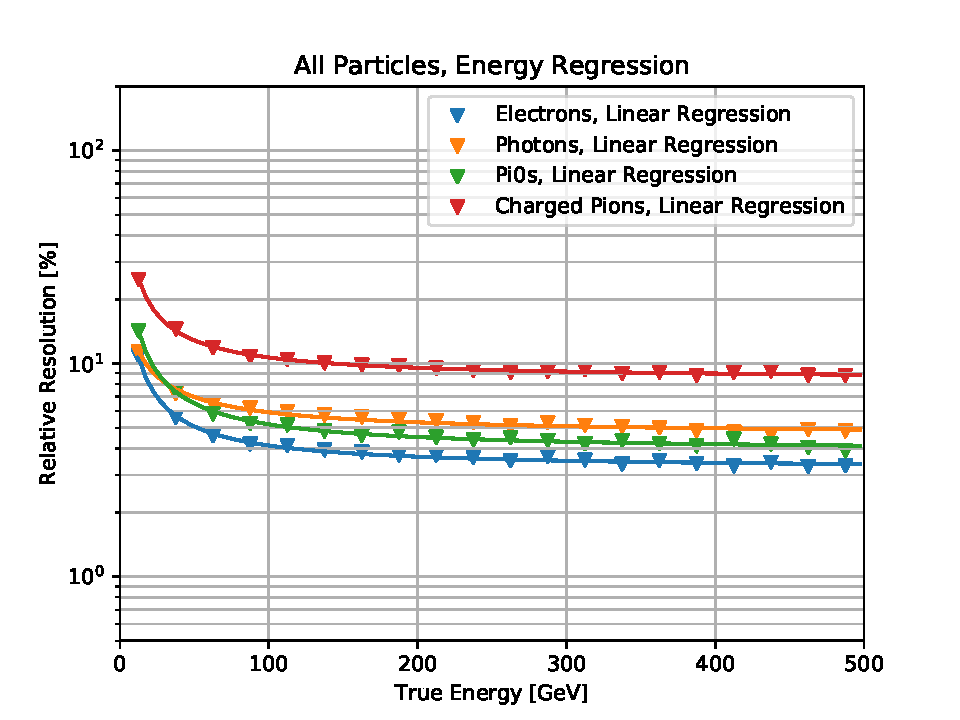
\includegraphics[width=0.45\textwidth]{Images/Calo/res_vs_E_allparts_linreg_fits.pdf}
\caption{Bias (left) and resolution (right) as a function of true energy for linear regression predictions of particle energy for the different particle types, trained on fixed-angle samples. \label{fig:reg_linreg}}
\end{figure}

We also investigated the use of BDTs for energy regression. This application has seen use in some LHC experiments (e.g., to study $H \rightarrow \gamma\gamma$ decays).  We used the XGBoost package in Python, with the following hyperparameters:

\begin{itemize}
\item maximum 1000 iterations, with early stopping if loss doesn't improve on the test set in 10 iterations
\item maximum tree depth of 3
\item minimum child weight of 1 (default)
\item learning rate $\eta = 0.3$ (default)
\end{itemize}

We used the following input features, as we found they gave good performance for electrons, photons, and \pizero. Adding the mean $z$ coordinate to the ECAL and HCAL total energies improved the energy resolution for all energy values, but in particular at high energy, as can be seen in Figure~\ref{fig:reg_xgb_ecalmoms}.

\begin{itemize}
\item total ECAL energy
\item total HCAL energy
\item mean $z$ coordinate of the ECAL shower
\end{itemize}

\begin{figure}[htbp]
\centering
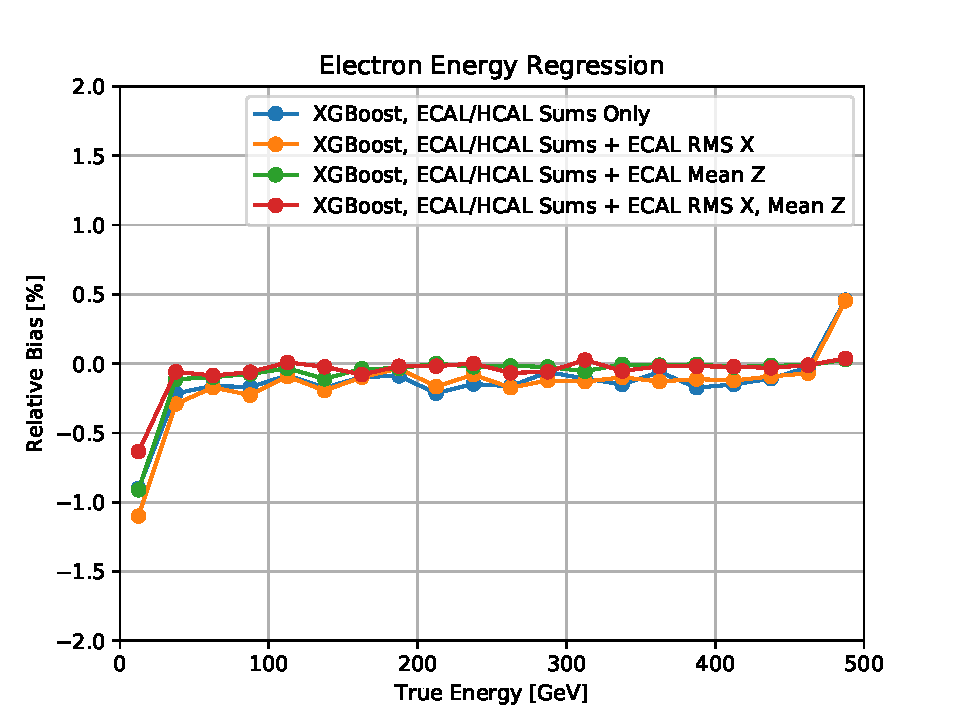
\includegraphics[width=0.45\textwidth]{Images/Calo/bias_vs_E_EleFixed_xgb_ecalmoms_zoom.pdf}
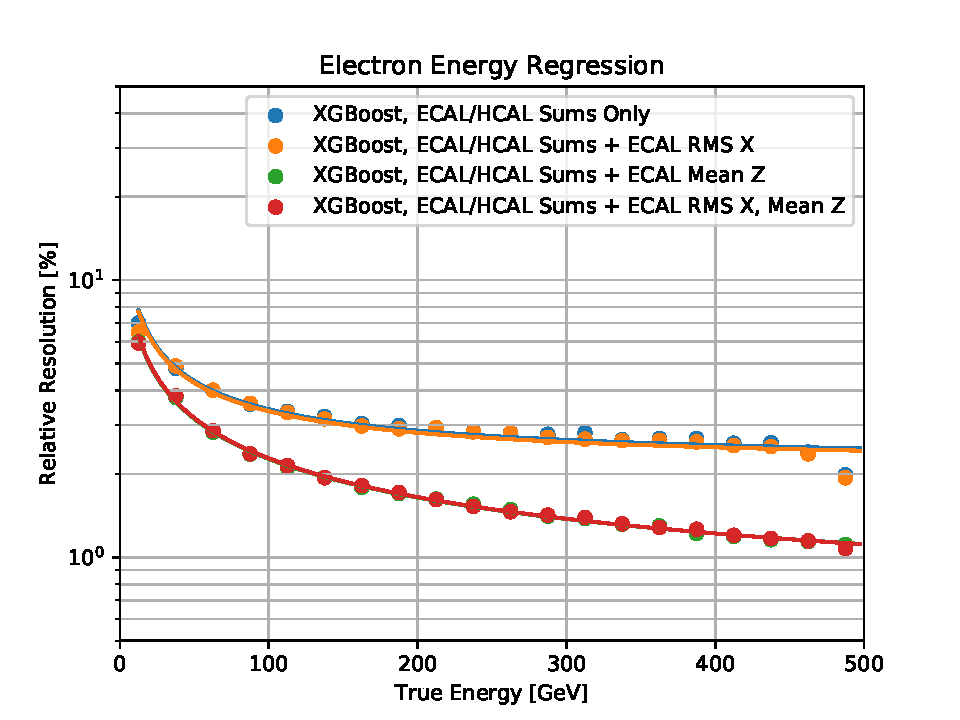
\includegraphics[width=0.45\textwidth]{Images/Calo/res_vs_E_EleFixed_xgb_ecalmoms_fits.pdf}
\caption{Bias (left) and resolution (right) as a function of true energy for the XGBoost regression predictions of particle energy, using different input features for electrons.\label{fig:reg_xgb_ecalmoms}}
\end{figure}

For \chpi, adding the following variables further improved the results:

\begin{itemize}
\item RMS in the $z$ direction of the ECAL shower
\item RMS in the $(x,y)$ plane of the HCAL shower
\item mean $z$ coordinate of the HCAL shower
\end{itemize}

In addition, for \chpi, around 0.5\% of events were found to have almost no reconstructed energy in the selected calorimeter window.  Including these events adversely affected the algorithm training, so they were removed for all the results shown in this and the following sections. Specifically, the raw ECAL+HCAL energy is required to be at least 30\% of the true generated energy.

The results of the XGBoost baseline are compared against linear regression in Figure~\ref{fig:reg_xgb_linreg}. The performance of XGBoost on electrons, photons, and \pizero\ is similar, achieving relative resolutions of about 6--8\% at the lowest energies and 1.0--1.1\% at the highest energies.  Compared to the baseline linear regression, the resolution improves by a factor of about two at low energy and three to four at high energy.  For \chpi, the resolution after XGBoost regression ranges between 20 and 5.4\%, with a relative improvement over linear regression of up to 40\% at high energy.

\begin{figure}[htbp]
\centering
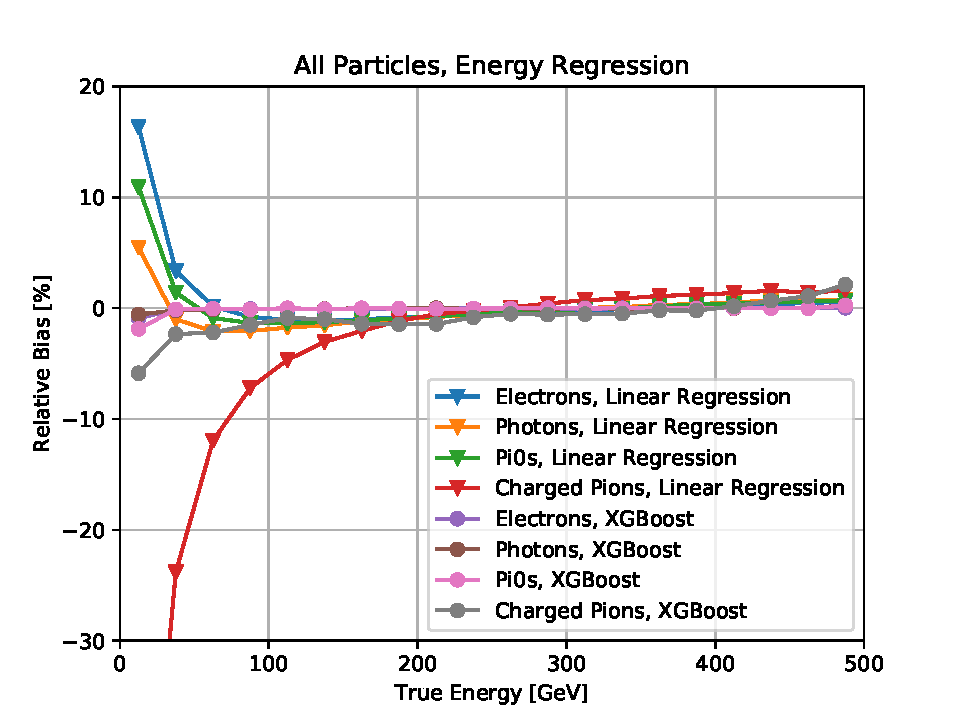
\includegraphics[width=0.45\textwidth]{Images/Calo/bias_vs_E_allparts_linreg_xgb.pdf}
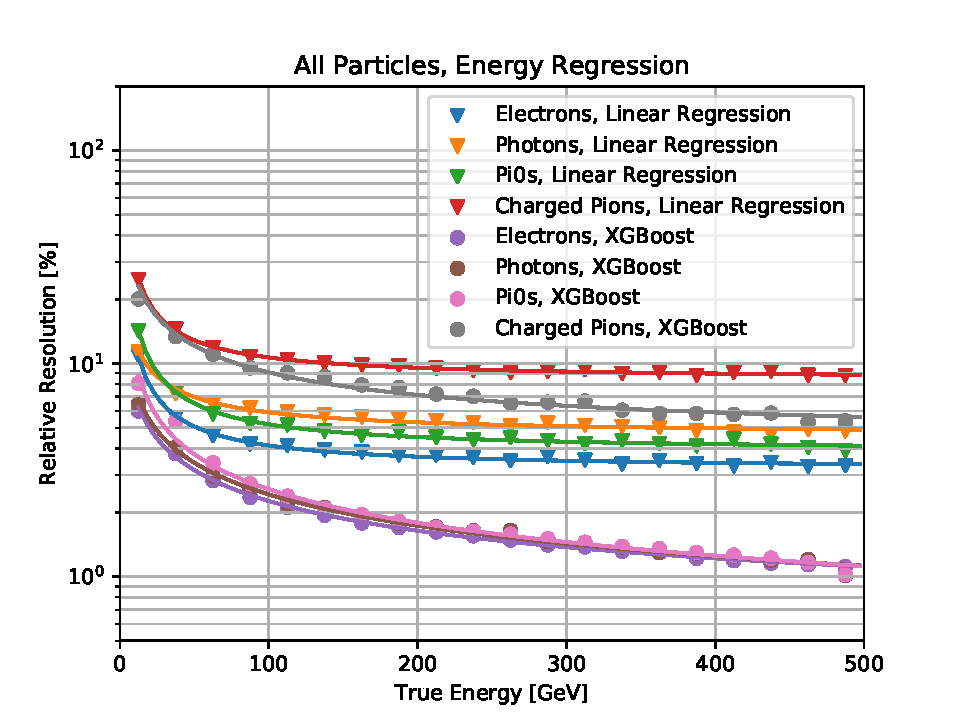
\includegraphics[width=0.45\textwidth]{Images/Calo/res_vs_E_allparts_linreg_xgb_fits.pdf}
\caption{Bias (left) and resolution (right) as a function of true energy for linear regression and XGBoost  predictions of particle energy for the different particle types.\label{fig:reg_xgb_linreg}}
\end{figure}

One drawback of using a BDT algorithm in a real-world setting is that it can not be used for energy values outside the range of the training set. That is, most tree algorithms do not perform extrapolation. This is an inherent disadvantage of the BDT when compared with the neural networks we present in this paper. However, despite this drawback, we use BDT results as a second baseline for comparison in our energy measurement task.

\section{Architecture and Training Details}

As mentioned before, we use a neural architecture which simultaneously performs both particle classification and energy regression. This combined network is trained using the ECAL and HCAL cell arrays as well as the total ECAL energy and total HCAL energy as inputs. The training loss function is written as the sum of a binary cross entropy for particle identification and a mean-square error loss for energy regression. Through experimentation, we found that multiplying the energy component of the loss function by a factor of 200 gave the best results, as it was easier to quickly achieve low loss values for energy regression.

We compare three different architectures for our reconstruction model:

\begin{itemize}
\item A dense (i.e, fully connected) neural network (DNN).
\item A 3D convolutional network (CNN).
\item A network based on GoogLeNet (GN)~\cite{GoogLeNet}, using layers of inception modules.
\end{itemize}

The architecture of each model is defined with a number of floating parameters (e.g. number of hidden layers), which are refined through hyperparameter optimization, as described in Section~\ref{sec:hpscan}. Each model returns three numbers. After applying a softmax activation, two of these elements are interpreted as the classification probabilities of the current two-class problem. The third output is interpreted as the energy of the particle.

Here we describe in detail the three model architectures:

\begin{itemize}
    \item In the DNN model we first flatten our ECAL and HCAL inputs into 1D arrays. We then concatenate these array along with the total ECAL energy, total HCAL energy, estimated $\phi$, and estimated $\eta$, for an array of total size $25 \times 25 \times 25 + 11 \times 11 \times 60 + 4 = 22889$ inputs. This array is fed as input to the first layer of the DNN, followed by a number of hidden layers each followed by a ReLU activation function and a dropout layer. The number of neurons per hidden layer and the dropout probability are identical for each relevant layer. The number of hidden layers, number of hidden neurons per layer, and dropout rate are hyperparameters, tuned as described in the next session.  Finally, we take the output from the last dropout layer, append the total energies and estimated angles again, and feed the concatenated array into a final hidden layer, which results in a three-element output. 
    \item The CNN architecture consists of one 3D convolutional layer for each of the ECAL and HCAL inputs, each followed by a ReLU activation function and a max pooling layer of kernel size $2 \times 2 \times 2$. The number of filters and the kernel size in the ECAL convolutional layer are treated as optimized hyperparameter (see next session). The HCAL layer is fixed at 3 filters with a kernel size of $2 \times 2 \times 6$. The two outputs are then flattened and concatenated along with the total ECAL and HCAL energies, as well as the estimated $\phi$ and $\eta$ coordinates of the incoming particle. The resulting 1D array is passed to a sequence of dense layers each followed by a ReLU activation function and dropout layer, as in the DNN model. The number of hidden layers and the number of neurons on each layer are considered as hyperparameters to be optimized. The output layer consists of three numbers, as for the DNN model. We found that adding additional convolutional layers to this model beyond the first had little impact on performance. This may be because a single layer is already able to capture important information about localized shower structure, and reduces the dimensionality of the event enough where a densely connected net is able to do the rest.
    \item The third model uses elements of the GoogLeNet~\cite{GoogLeNet} architecture. This network processes the ECAL input array with a 3D convolutional layer with 192 filters, a kernel size of 3 in all directions, and a stride size of 1. The result is batch-normalized and sent through a ReLU activation function. This is followed by a series of inception and MaxPool~\cite{conv} layers of various sizes, as will be described in detail below. The output of this sequence is concatenated to the total ECAL energy, the total HCAL energy, the estimated $\phi$ and $\eta$ coordinates, and passed to a series of dense layers like in the DNN architecture, to return the final three outputs. The number of neurons in the final dense hidden layer is the only architecture-related hyperparameter for the GN model. Due to practical limitations imposed by memory constraints, this model does not take the HCAL 3D array as input. This limitation has a small impact on the model performance, since the ECAL array carries the majority of the relevant information for the problems at hand.
\end{itemize}

On all models, the regression task is facilitated by using skip connections to directly append the input total ECAL and HCAL energies to the last layer. The impact of this architecture choice on regression performance is described later in this chapter. In addition to using total energies, we also tested the possibility of using 2D projections of the input energy arrays, summing along the $z$ dimension (detector depth). This choice resulted in worse performance (as described later in this chapter) and was discarded.

\subsection*{GoogLeNet-Based Model Architecture Details}

In our GoogLeNet architecture, we use inception modules. In these modules, inputs go through four separate branches and are then concatenated together. For an inception layer denoted as Inception(A, B, C, D, E, F, G) the branches are defined as follows:

\begin{itemize}
    \item Branch 1: A simple $1 \times 1 \times 1$ convolution, taking A input channels to B output channels. This is followed by a batch normalization and a ReLU activation function.
    \item Branch 2: A $1 \times 1 \times 1$ convolution followed by a $3 \times 3 \times 3$ convolution. The first convolution takes A input channels to C output channels, followed by batch normalization and ReLU. This then goes to the next convolution layer, which outputs D channels using a kernel of size $3 \times 3 \times 3$. This is again followed by batch normalization and ReLU.
    \item Branch 3: A $1 \times 1 \times 1$ convolution followed by a $5 \times 5 \times 5$ convolution. The details are the same as for the other branches, but the first convolution takes A input channels to E output channels, and the next convolution outputs F channels.
    \item Branch 4: A max pool of kernel size $3 \times 3 \times 3$ is followed by a convolution of kernel size $1 \times 1 \times 1$ that takes A input channels to G output channels. This is followed once again by batch normalization and ReLU.
\end{itemize}

Here are full details for each layer of the GoogLeNet-based architecture:

\begin{itemize}
    \item Apply instance normalization to ECAL input.
    \item Convolution with 3D kernel of size 3, going from 1 input channel to 192 channels, with a padding of 1. This is followed by batch normalization and ReLU.
    \item Inception(192,  64,  96, 128, 16, 32, 32)
    \item Inception(256, 128, 128, 192, 32, 96, 64)
    \item Max pooling with a 3D kernel of size 3, a stride of 2, and padding of 1.
    \item Inception(480, 192,  96, 208, 16,  48,  64)
    \item Inception(512, 160, 112, 224, 24,  64,  64)
    \item Inception(512, 128, 128, 256, 24,  64,  64)
    \item Inception(512, 112, 144, 288, 32,  64,  64)
    \item Inception(528, 256, 160, 320, 32, 128, 128)
    \item Max pooling with a 3D kernel of size 3, a stride of 2, and padding of 1.
    \item Inception(832, 256, 160, 320, 32, 128, 128)
    \item Inception(832, 384, 192, 384, 48, 128, 128)
    \item Average pooling with a 3D kernel of size 7 and a stride of 1.
    \item The output array is flattened and concatenated with input $\phi$, $\eta$, total ECAL energy, and total HCAL energy.
    \item A densely connected layer with 1024 outputs, followed by ReLU.
    \item The output array is once again concatenated with the same input values.
    \item A final densely connected layer outputs 5 values, as in the architectures of the other two models.
\end{itemize}

The full architecture is shown in Figure~\ref{fig:gn_with_inceptin}.

\begin{figure}[htbp]
\centering
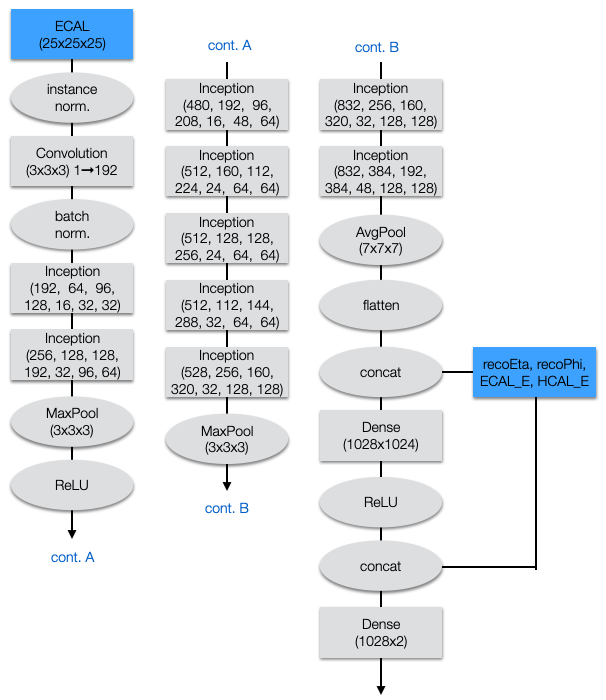
\includegraphics[width=0.45\textwidth]{Images/Calo/GN_architecture.png}
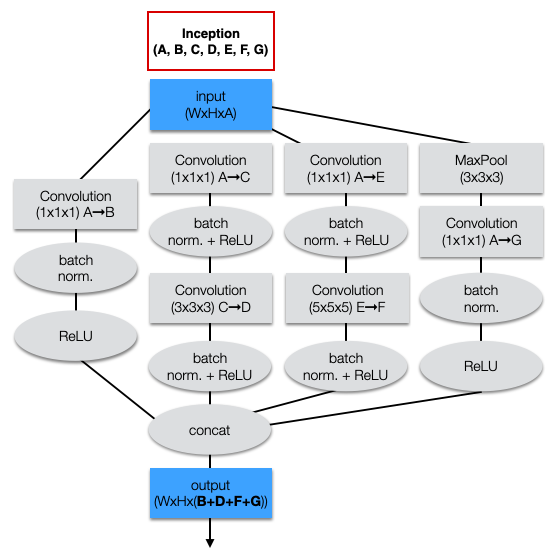
\includegraphics[width=0.45\textwidth]{Images/Calo/inception_architecture.png}
\caption{GoogLeNet-based architecture (top) and component inception architecture (bottom).
}
\label{fig:gn_with_inceptin}
\end{figure}

\subsection*{Use of HCAL in Reconstruction}

Since the GoogLeNet architecture was quite large and required significant memory usage and computational power, we decided to investigate the possibility of leaving out HCAL cell-level information, since most of the particle shower occurs in the ECAL. After optimizing our DNN, we took our best-performing DNN architecture and ran ten training sessions with HCAL information, and ten training sessions without HCAL. Averaged training curves from these runs are shown in Figures~\ref{fig:HCAL_study_elechpi} and~\ref{fig:HCAL_study_gammapi0}. These studies demonstrated that including the HCAL caused little to no improvement in classification accuracy. For memory purposes, we thus kept HCAL cell-level information out of our GN architecture. Summed HCAL energy was still fed as an input to the combined classification-regression net, for use in energy regression.

We must note here that though HCAL information is useful for particle reconstruction in general, the reason we do not see much use for it here is because we are mostly looking at events where the majority of energy is deposited in the ECAL. This is particularly true due to the HCAL/ECAL ratio we have applied to electron/charged pion events.

\begin{figure}[htbp]
\centering
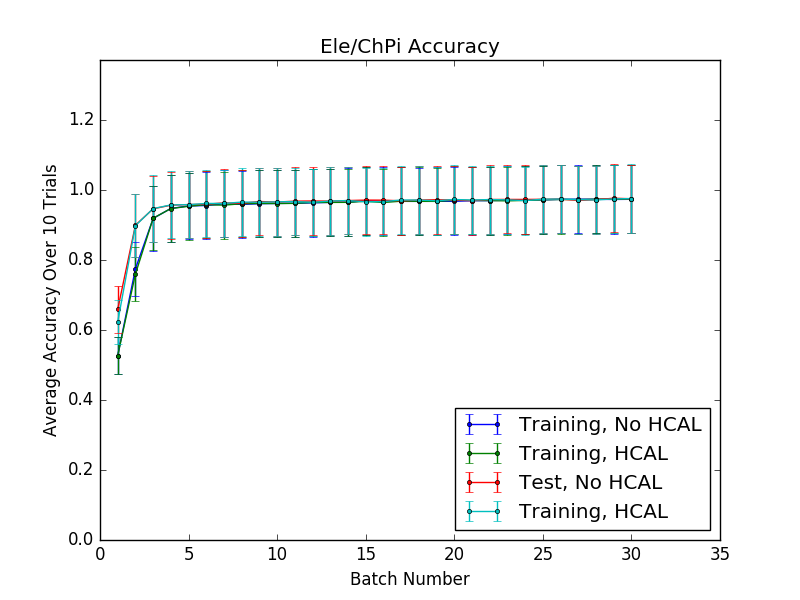
\includegraphics[width=0.45\textwidth]{Images/Calo/HCAL_study_elechpi_accuracy.png}
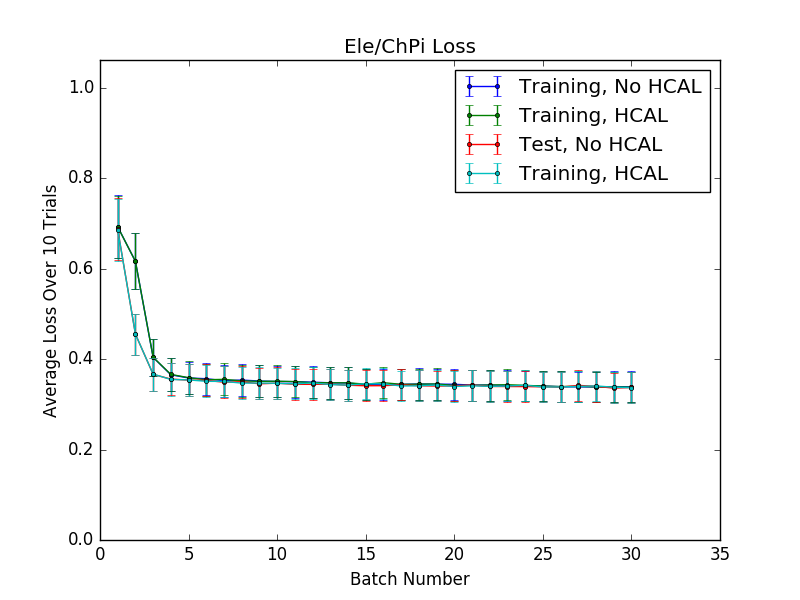
\includegraphics[width=0.45\textwidth]{Images/Calo/HCAL_study_elechpi_loss.png}
\caption{Accuracy and loss curves for electron/charged pion classification, with and without HCAL cells, using best DNN architecture.}
\label{fig:HCAL_study_elechpi}
\end{figure}

\begin{figure}[htbp]
\centering
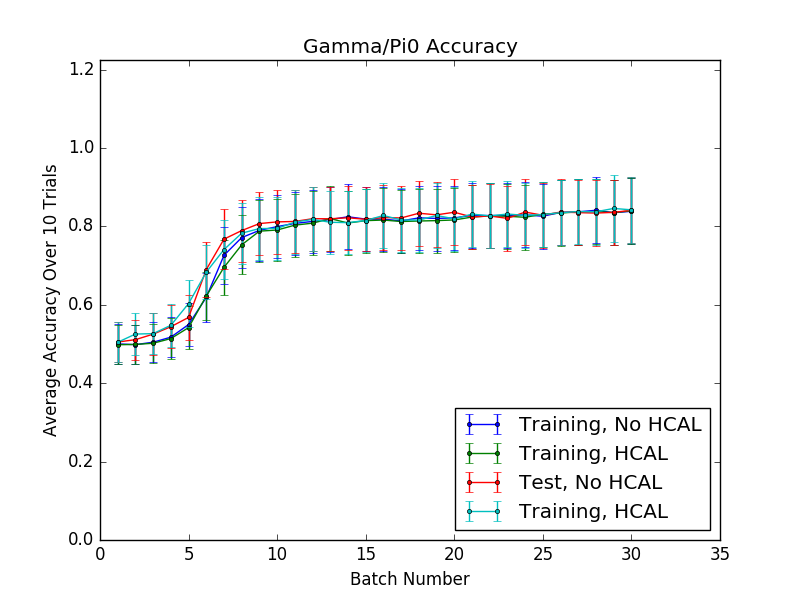
\includegraphics[width=0.45\textwidth]{Images/Calo/HCAL_study_gammapi0_accuracy.png}
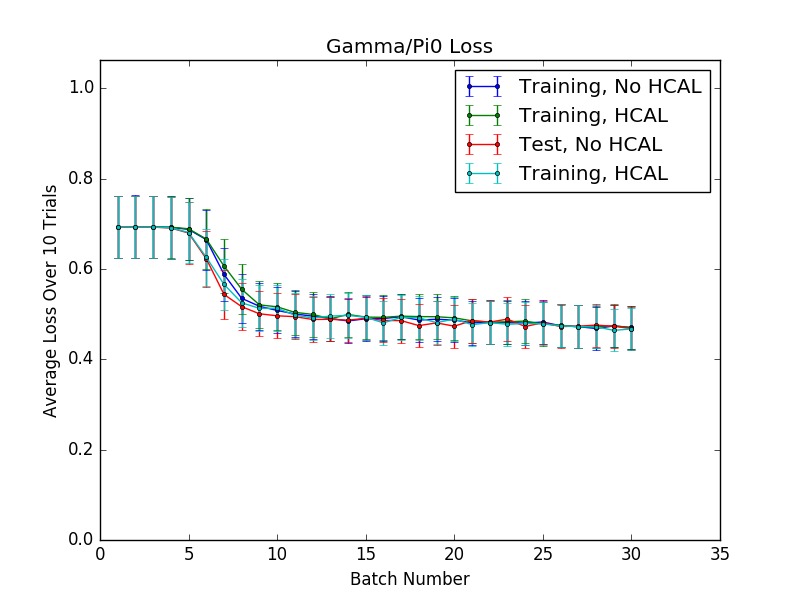
\includegraphics[width=0.45\textwidth]{Images/Calo/HCAL_study_gammapi0_loss.png}
\caption{Accuracy and loss curves for photon/neutral pion classification, with and without HCAL cells, using best DNN architecture.}
\label{fig:HCAL_study_gammapi0}
\end{figure}

\subsection*{Regression with Large Sample Windows}

We saw earlier that classification was not affected by a larger calorimeter window. We wanted to see the effects of using a smaller window on reconstruction as well. We found that for both DNN and CNN, to achieve the best performance for energies above 150~GeV, a minimum $(x,y)$ size of 25x25 in the ECAL and 5x5 in the HCAL is needed. For energies below 150~GeV, the optimal performance is observed for a window size of 51x51 in the ECAL and 11x11 in the HCAL. This is presumably due to wider showers at low energy.  The impact of the choice of window size is shown for DNN in Figure~\ref{fig:reg_dnn_numcells}, with the results for CNN being similar.  Drawbacks to the larger window size, however, include larger files, more memory usage, and that training takes about 5 times longer per epoch.

\begin{figure}[htbp]
\centering
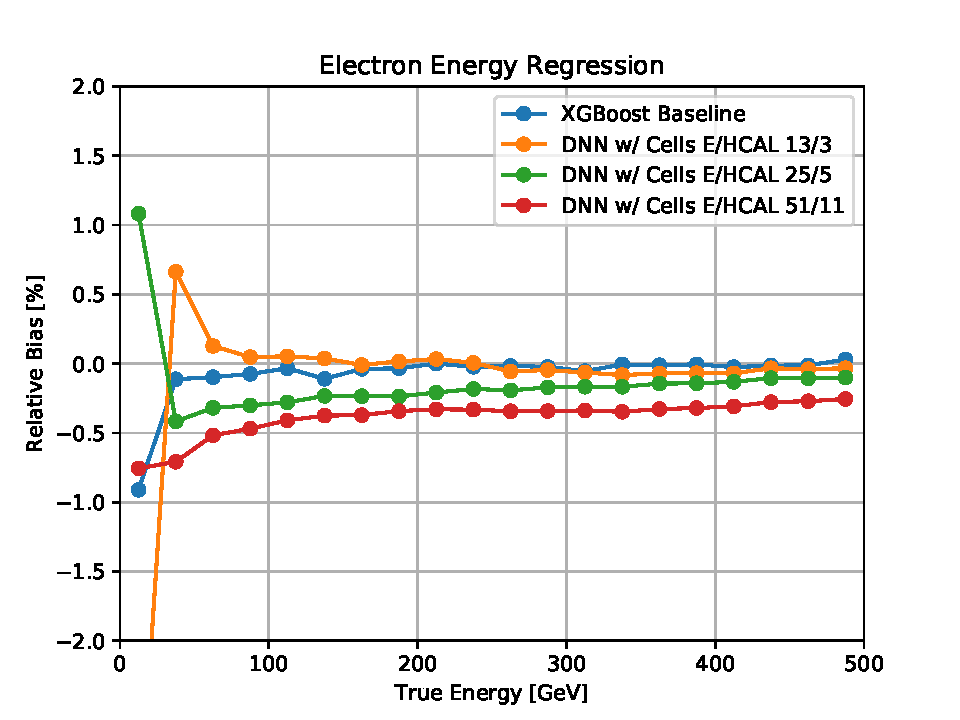
\includegraphics[width=0.45\textwidth]{Images/Calo/bias_vs_E_EleFixed_nn_numcells_zoom.pdf}
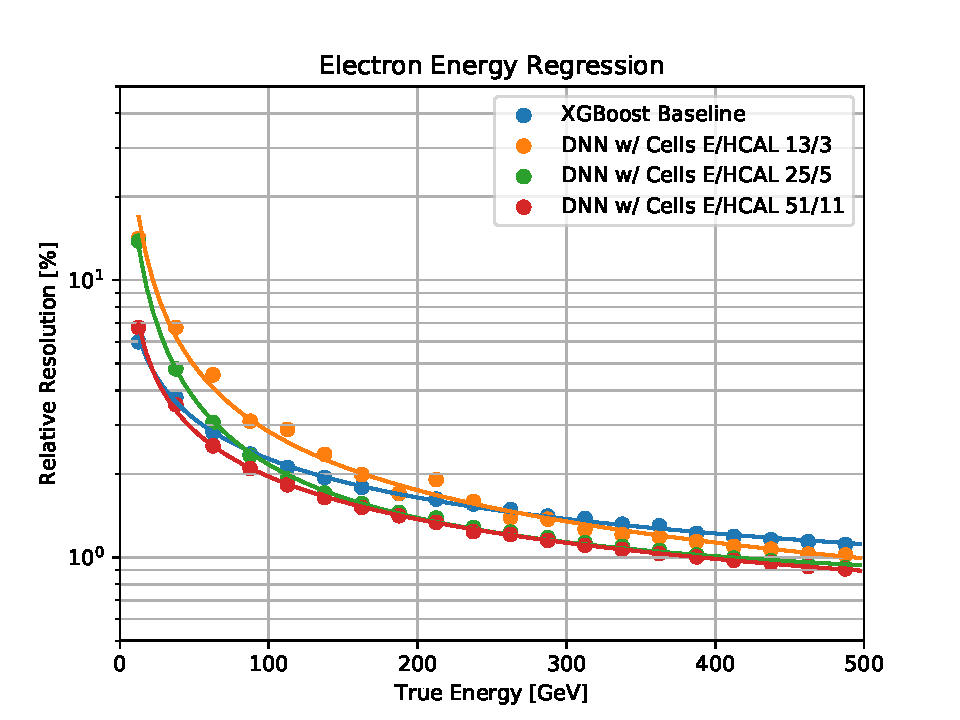
\includegraphics[width=0.45\textwidth]{Images/Calo/res_vs_E_EleFixed_nn_numcells_fits.pdf}
\caption{Bias (left) and resolution (right) as a function of true energy for DNN energy predictions for electrons, with varying input window sizes.
}
\label{fig:reg_dnn_numcells}
\end{figure}

Showers for \chpi\ were observed to be wider than the other particle types, especially at low energies, and so we compare the effect of the calorimeter window size choice for \chpi\ in Figure~\ref{fig:reg_nn_numcells_chpi_large_window}. The wider window of 51x51 in $(x,y)$ in the ECAL and 11x11 in the HCAL gives better performance, especially at the lowest energies where the resolution is improved by a factor of about 2 over the smaller window size (25x25 ECAL, 5x5 HCAL).

\begin{figure}[htbp]
\centering
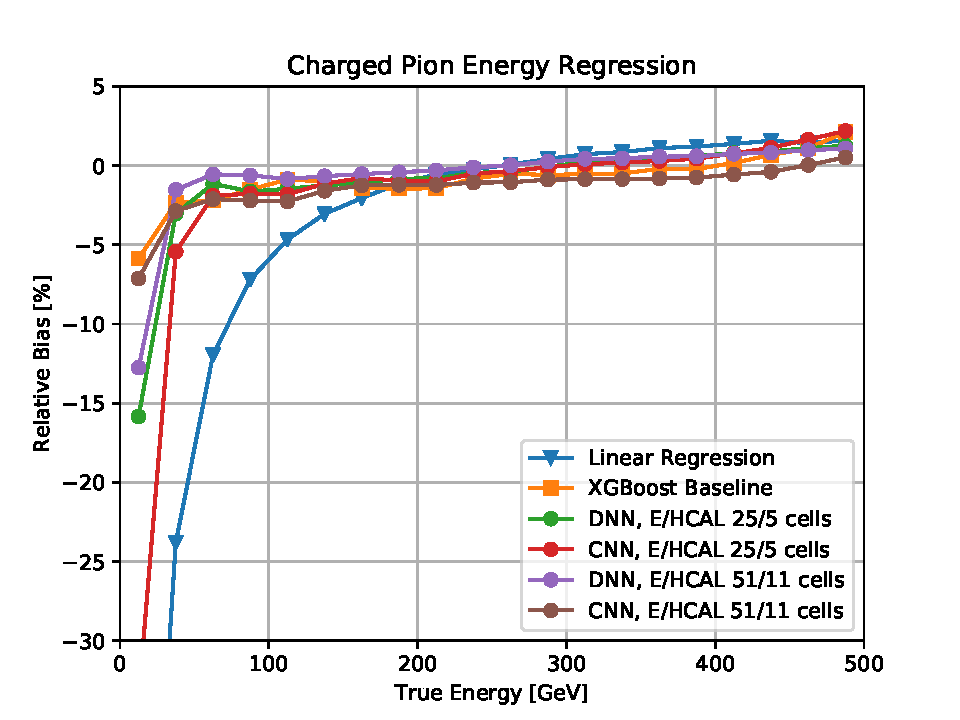
\includegraphics[width=0.45\textwidth]{Images/Calo/bias_vs_E_ChPiFixed_Cut30_nn_numcells.pdf}
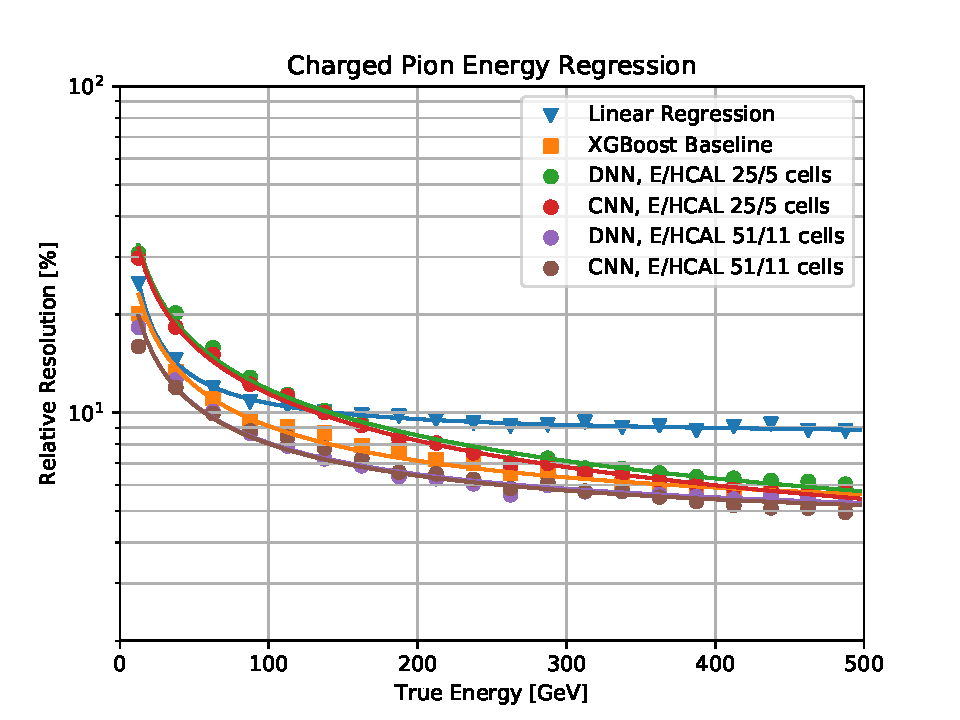
\includegraphics[width=0.45\textwidth]{Images/Calo/res_vs_E_ChPiFixed_Cut30_nn_numcells_fits.pdf}
\caption{Bias (left) and resolution (right) as a function of true energy for energy predictions for \chpi, comparing calorimeter window sizes for the CNN and DNN models.
}
\label{fig:reg_nn_numcells_chpi_large_window}
\end{figure}

Overall, though the larger window did make a bit of difference, the improvement was not large enough to overcome the downsides, and we decided to stick with smaller windows for training.

\subsection*{Skip Connections}

A design choice that improved convergence time, and improved performance for the CNN, was including ``skip connections'' for the total ECAL and HCAL energies in the network.  In addition to the individual cell energy values, the total ECAL and HCAL energy values are given as inputs to both the first dense layer and to the last output layer.  The weights for these energy values are initialized to 1, as linear regression with coefficients near 1 is observed to reasonably reproduce the true energy values.  The impact of adding skip connections on performance using a CNN architecture for a fixed number of 5 training epochs is shown in Figure~\ref{fig:reg_cnn_skip}.

\begin{figure}[htbp]
\centering
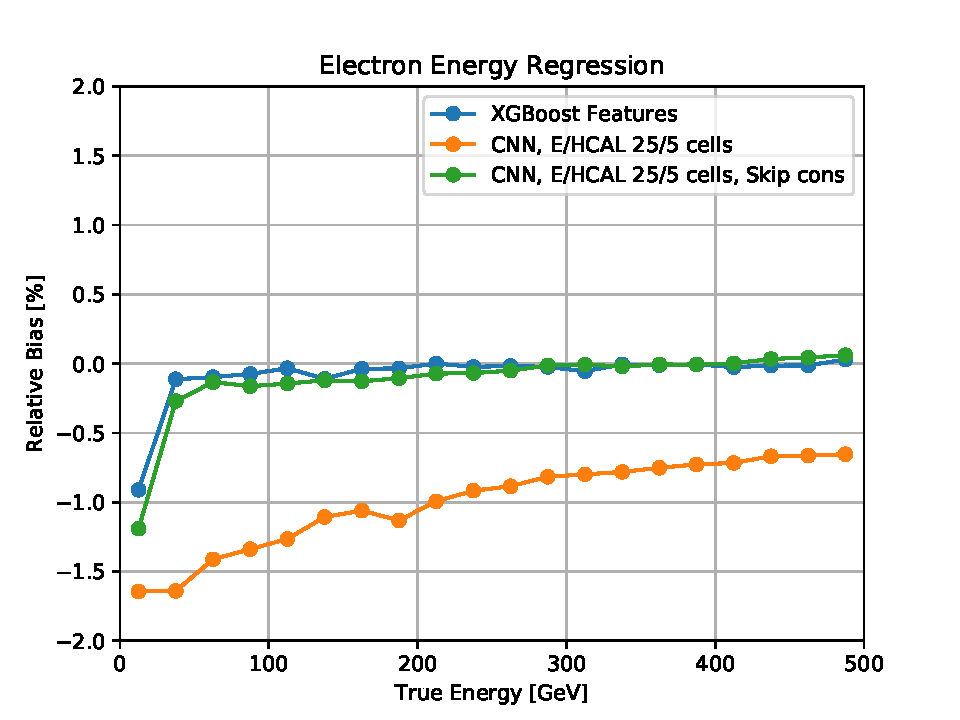
\includegraphics[width=0.45\textwidth]{Images/Calo/bias_vs_E_EleFixed_cnn_skip_zoom.pdf}
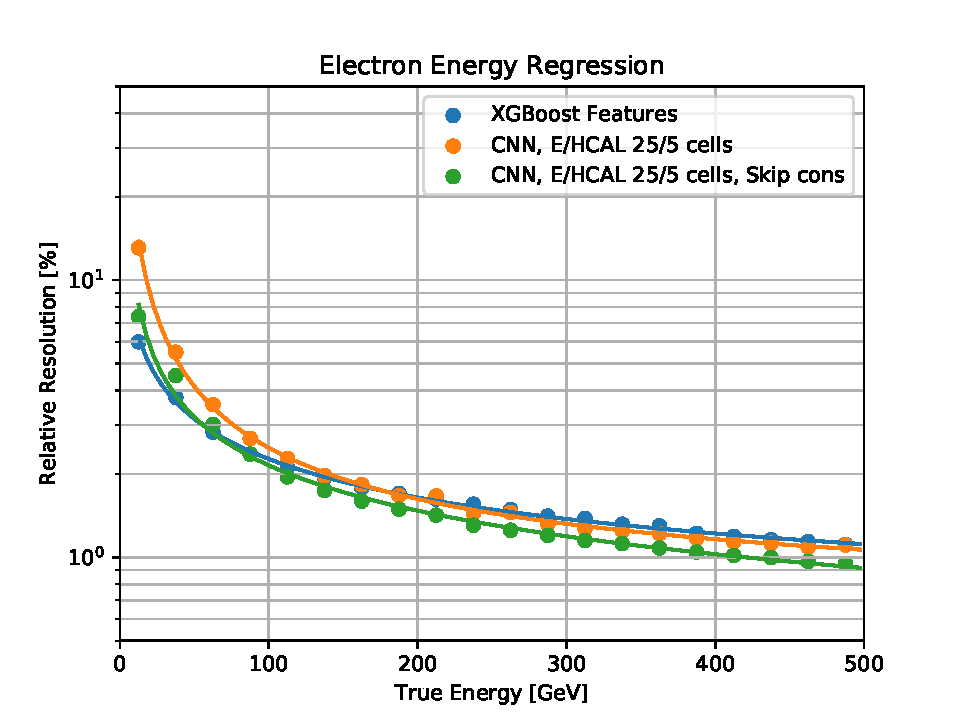
\includegraphics[width=0.45\textwidth]{Images/Calo/res_vs_E_EleFixed_cnn_skip_fits.pdf}
\caption{Bias (left) and resolution (right) as a function of true energy for CNN energy predictions for electrons, with or without skip connections in the architecture.
}
\label{fig:reg_cnn_skip}
\end{figure}

\subsection*{Training Using Energy Summed in z}

For regression, we tried using only the energy summed in layers in the $z$ direction, instead of the full array of cell energies, as the mean $z$ coordinate was seen to be the most important additional feature in the XGBoost baseline.  The performance is better than the XGBoost baseline at high energies but worse than using the full cell-level information, as shown in Figure~\ref{fig:reg_dnn_inputs}.

\begin{figure}[htbp]
\centering
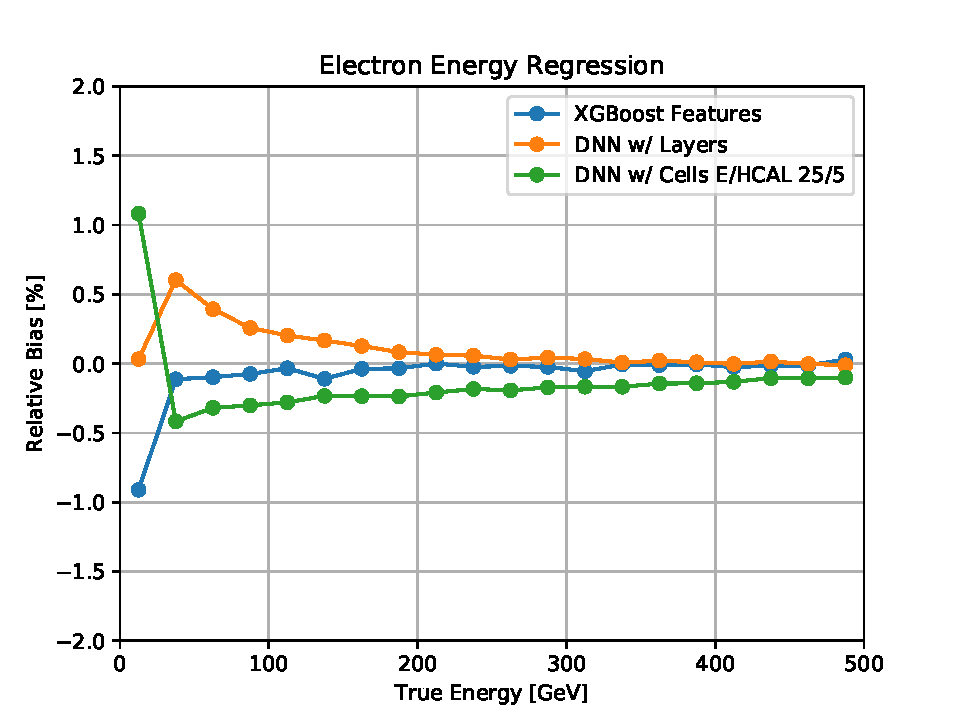
\includegraphics[width=0.45\textwidth]{Images/Calo/bias_vs_E_EleFixed_nn_inputs_zoom.pdf}
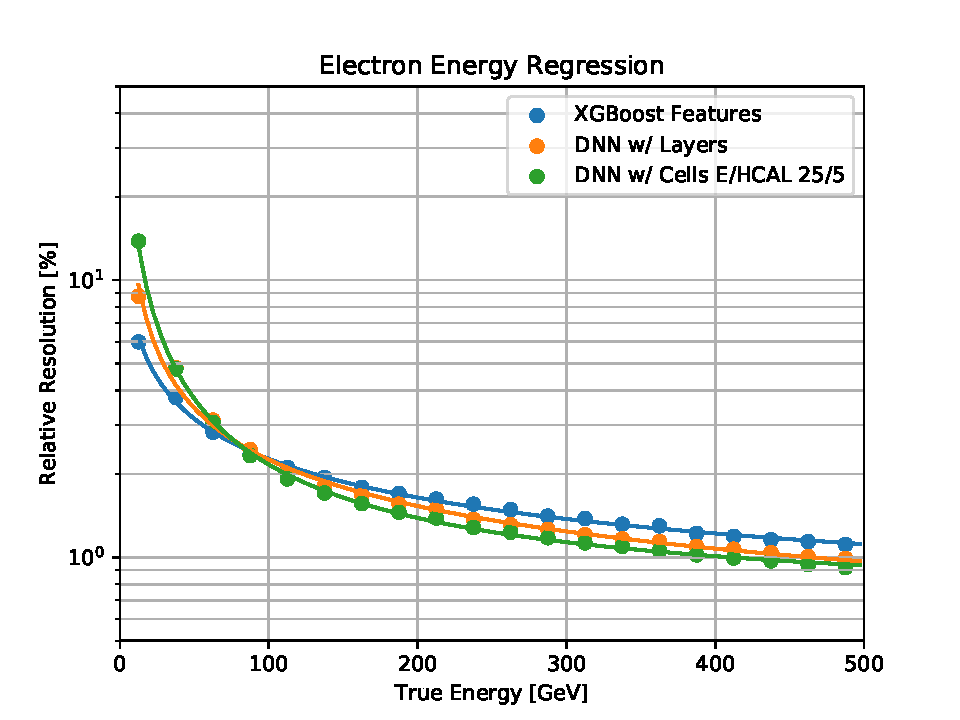
\includegraphics[width=0.45\textwidth]{Images/Calo/res_vs_E_EleFixed_nn_inputs_fits.pdf}
\caption{Bias (left) and resolution (right) as a function of true energy for DNN energy predictions for electrons, using as input either the energy summed in layers of $z$, or the full cell information.\label{fig:reg_dnn_inputs}}
\end{figure}

\section{Hyperparameter Scans}\label{sec:hpscan}

In order to fine-tune our models, we scanned over a hyperparameter space for each architecture. In addition to architecture parameters, learning rate and decay rate were additional hyperparameters for each architecture. For simplicity, we used classification accuracy for the $\gamma$ vs. $\pi^0$ problem as a metric to determine the overall best hyperparameter set for each architecture. This is because a model optimized for this task was found to generate good results for the other tasks as well, since $\gamma$ vs. $\pi^0$ classification was found to be the most difficult problem.

Training was performed at each hyperparameter point ten times, in order to obtain an estimate of the uncertainty associated with each quoted performance value. For each scan point, the DNN and CNN architectures trained on 400,000 events, using another sample of 400,000 events for testing. DNN and CNN scan points trained for three epochs each, taking about seven hours each. GN trained on 100,000 events and tested on another 100,000. Due to a higher training time, each GN scan point only trained for a single epoch, taking about twenty hours.

For CNN and DNN training, we used batches of 1,000 events when training. However, due to GPU memory limitations, we could not do the same with GN. Instead, we split each batch into 100 minibatches of ten events each. A single minibatch was loaded on the GPU at a time, and gradients were added up after back-propagation. We waited until after each batch was fully calculated to update network weights using the combined gradients. The best settings were found to be as follows:

\begin{itemize}
    \item For DNN, 4 hidden layers, 512 neurons per hidden layer, a learning rate of 0.0002, decay rate of 0, and a dropout probability of 0.04.
    \item For CNN, 4 hidden layers and 512 neurons per hidden layer, a learning rate of 0.0004, decay rate of 0, a dropout probability of 0.12, 6 ECAL filters with a kernel size of $6 \times 6 \times 6$.
    \item For GN, 1024 neurons in the hidden layer, 0.0001 learning rate, and 0.01 decay rate. 
\end{itemize}
%For CNN and GN, a very mild dependence on the number of neurons per hidden layer is observed. 

\begin{figure*}[htbp]
\centering
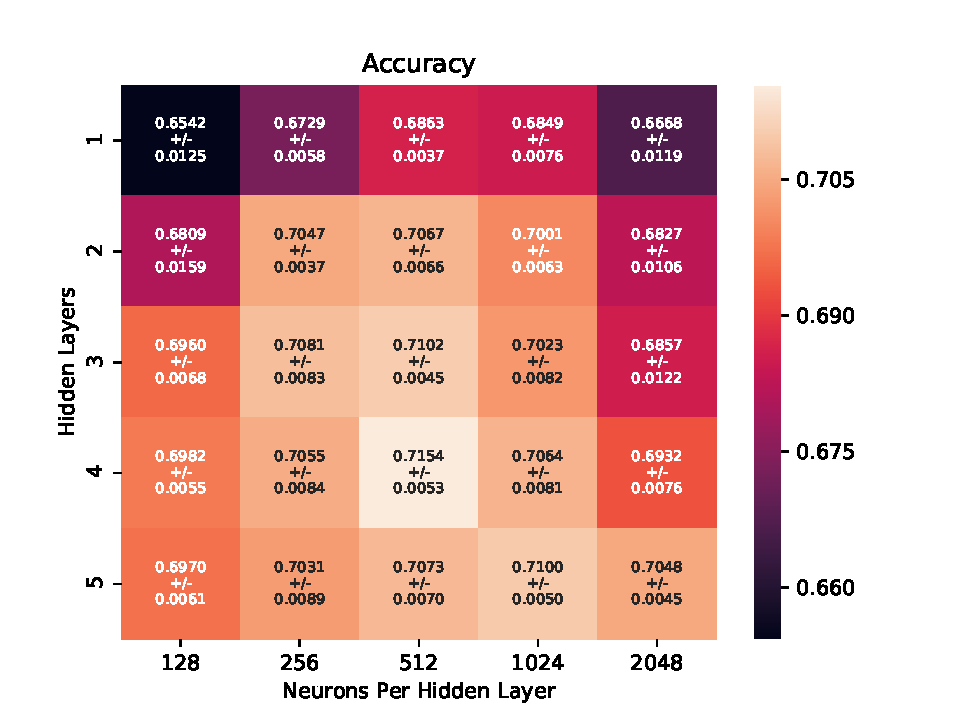
\includegraphics[width=0.45\textwidth]{Images/Calo/DNN_hl_nhl.pdf}
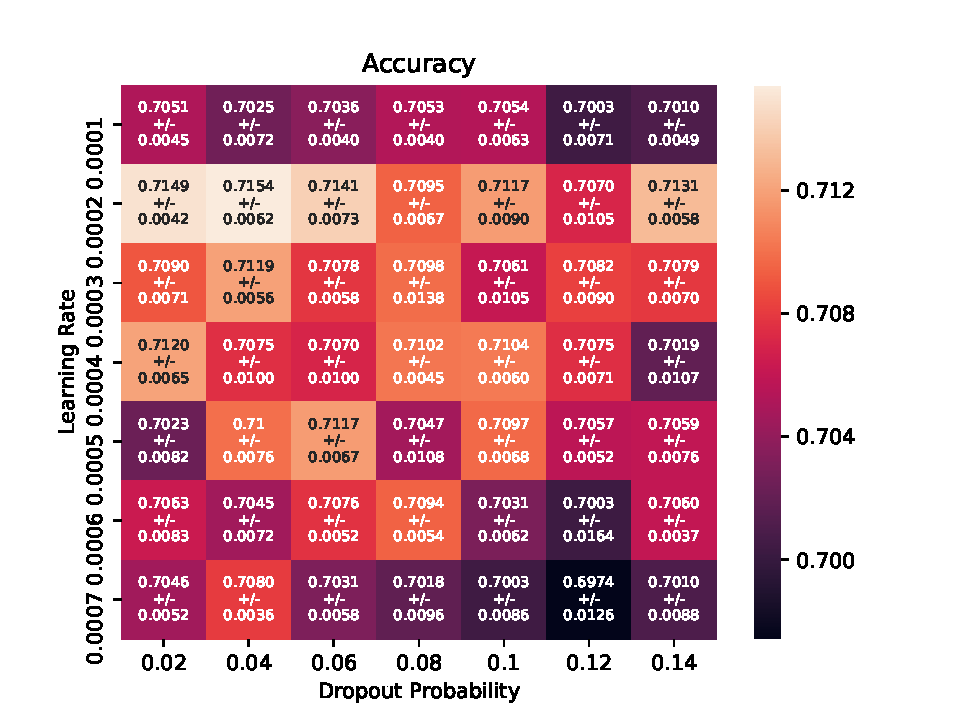
\includegraphics[width=0.45\textwidth]{Images/Calo/DNN_lr_dp.pdf} \\
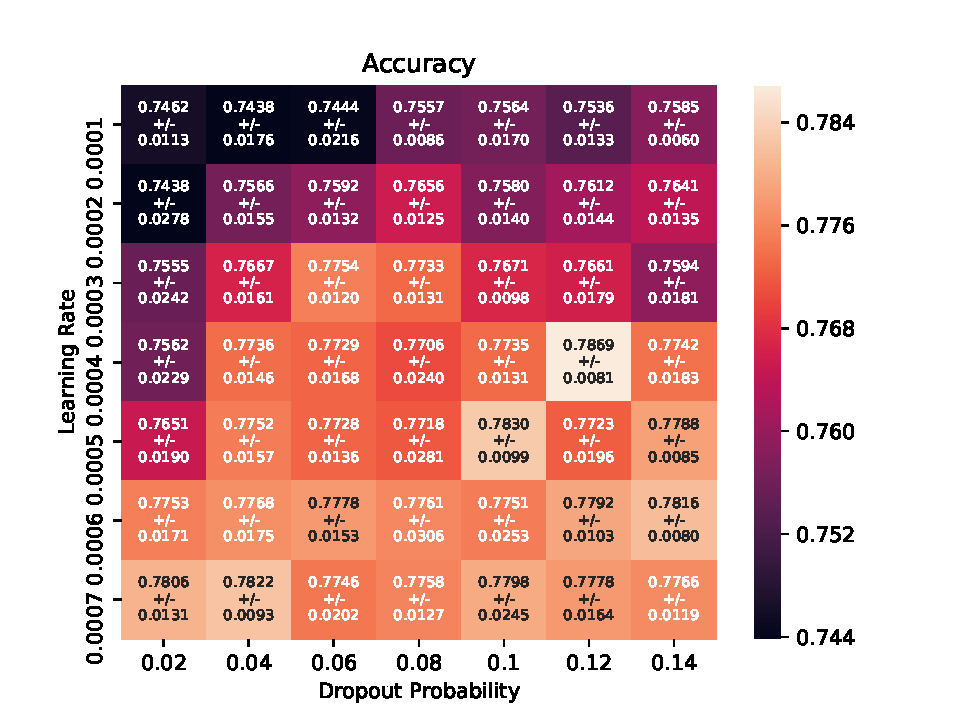
\includegraphics[width=0.45\textwidth]{Images/Calo/CNN_lr_dp.pdf}
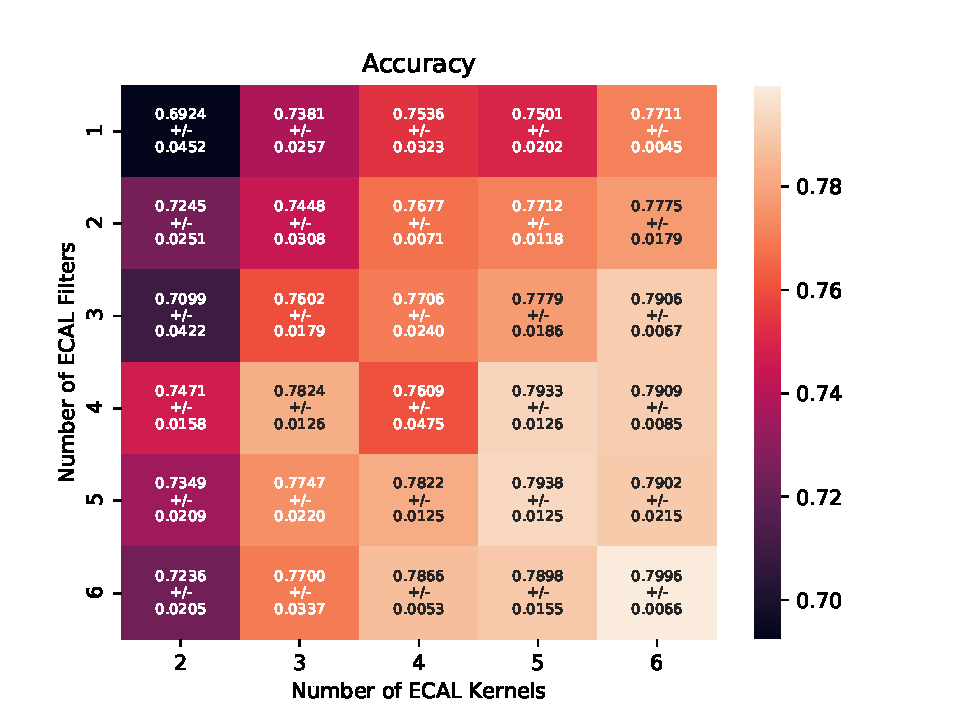
\includegraphics[width=0.45\textwidth]{Images/Calo/CNN_nECALfilt_nECALkern.pdf} \\
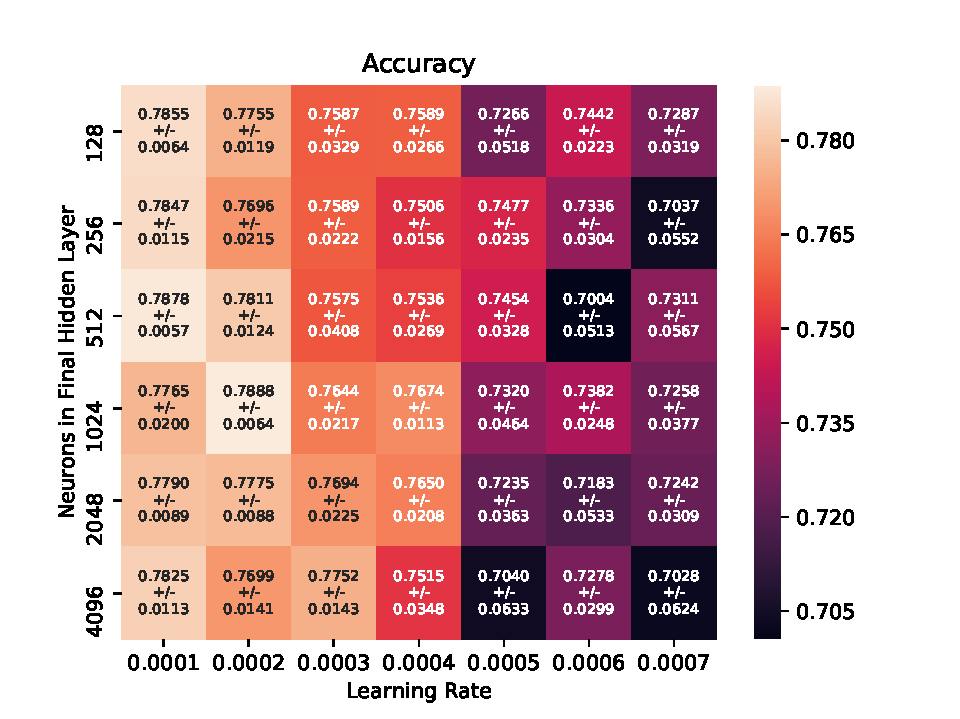
\includegraphics[width=0.45\textwidth]{Images/Calo/GN_nhl_lr.pdf}
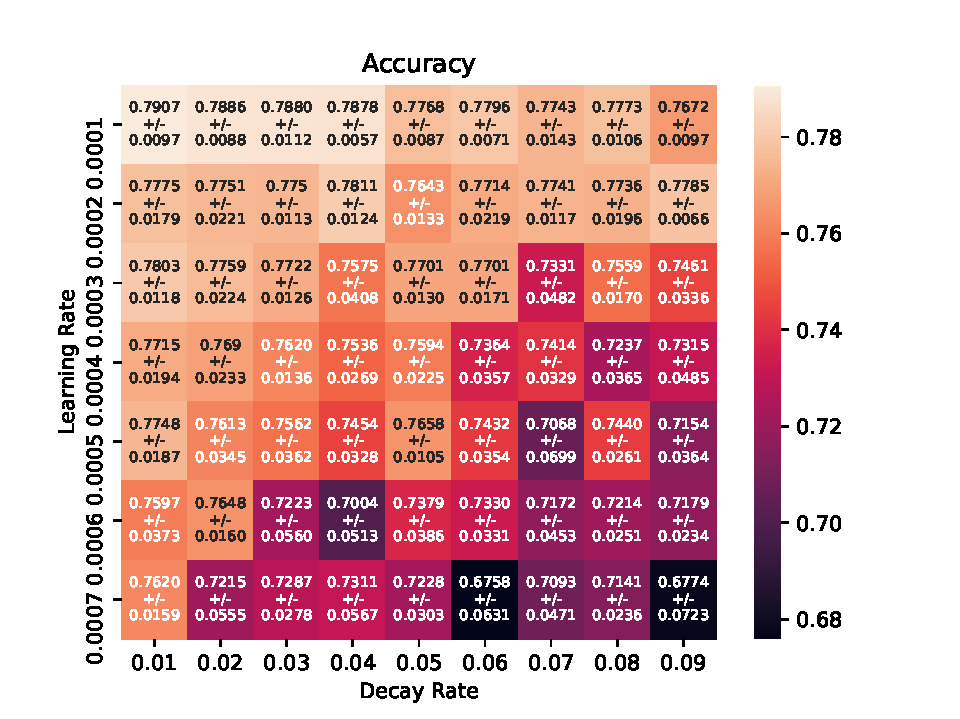
\includegraphics[width=0.45\textwidth]{Images/Calo/GN_lr_dr.pdf}
\caption{Selected hyperparameter scan results for DNN (top), CNN (center), and the GoogLeNet-based architecture (bottom). In each figure, the classification accuracy is displayed as a function of the hyperparameters reported on the two axes.}
\label{fig:scan_hyperparameter}
\end{figure*}

The DNN, CNN, and GN-based models had 9823774 ($\sim$10M), 3003692 ($\sim$3M), and 14956286 ($\sim$15M) trainable parameters respectively after the hyperparameter scans.

Selected hyperparameter scan slices are shown in Figure~\ref{fig:scan_hyperparameter}. 
These 2D scans were obtained setting all values besides the two under consideration (i.e., those on the axes) to be fixed at default values: a dropout rate of 0.08, a learning rate of 0.0004, a decay rate of 0.04, three dense layers for CNN and DNN, and 512 neurons per hidden layer. For GN, the default number of ECAL filters was 3, with a kernel size of 4.
%An ECAL window size of 25 was used in all instances, to allow fair comparison between DNN, CNN, and GN, as larger ECAL sizes posed a memory problem when training GN.

After performing the hyperparameter scan, we trained each architecture using its optimal hyperparameters for a greater number of epochs. The evolution of the training and validation accuracy as a function of the batch number for these extended trainings is shown in Figure~\ref{fig:training_curves_comparison_gamma_pi0}.

\begin{figure}[htbp]
\centering
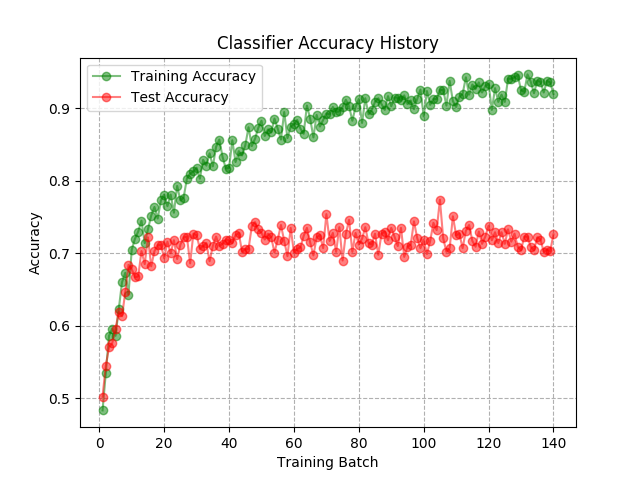
\includegraphics[width=0.45\textwidth]{Images/Calo/DNN_accuracy_batches_long.png}
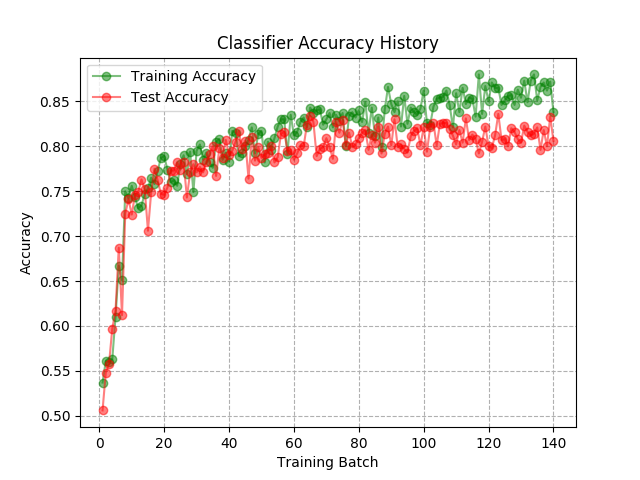
\includegraphics[width=0.45\textwidth]{Images/Calo/CNN_accuracy_batches_long.png}
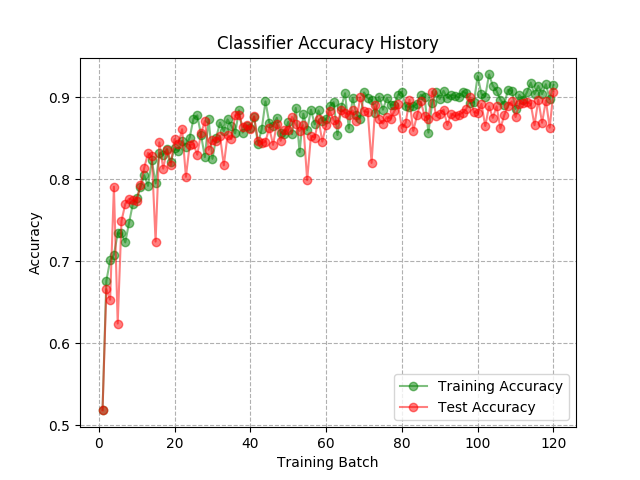
\includegraphics[width=0.45\textwidth]{Images/Calo/GN_accuracy_batches_long.png}
\caption{Training curves for best DNN (top), CNN (middle), and GoogLeNet (bottom) hyperparameters, trained on variable-angle $\gamma$/$\pi^0$ samples. We see that the DNN over-trains quickly and saturates at a relatively low accuracy, while the CNN takes longer to over-train and reaches a higher accuracy, and GoogLeNet performs best of all. Each 400 batches corresponds to a single epoch.}
\label{fig:training_curves_comparison_gamma_pi0}
\end{figure}